\section{Theoretical Background}

In the following section the theoretical knowledge necessary to understand and perform the experiment will be discussed.

\subsection{Maxwell Equations}

Light is described by electromagnetic waves with a wavelength in a range of $400-800\,\mathrm{nm}$. The behavior and propagation of electromagnetic waves is governed by Maxwell equations which in its source-free form are given as follows \cite{demtroeder2}:

\begin{align}
	\nab \vec{E}&=0\\
	\nab \vec{B}&=0\\
	\nab\times\vec{E}&=-\del[\vec B]{t}\\
	\nab\times\vec{B}&=\frac1{c^2}\del[\vec B]{t}\text{ ,}
\end{align}
from which we obtain the electromagnetic wave equations:
\begin{align}
	\Delta \vec{E} + \frac{1}{c^2} \ddot{\vec{E}}&= 0\\
	\Delta \vec{B} + \frac{1}{c^2} \ddot{\vec{B}}&= 0\text{ ,}
\end{align}

where the electric field is denoted by E and the magnetic field by B respectively. It can easily be shown that the solutions of these differential equations are given by waves which gives the equations their name. In the following we will only consider the electric field when talking about waves for simplicity. Two particular solutions, plane and spherical waves, will be discussed in more detail in the following paragraphs.
\paragraph{Plane Waves}

This solution of Maxwell equations describes a monochromatic, homogeneous plane wave. The amplitude of such a wave will be given by a sinusoidal function of the position r and time t. Practically ideal plane waves aren't possible as they would have to fill all space and be of infinite extent in order to propagate as plane waves. However, plane waves often yield a good approximation locally. Plane waves are described as follows:

\begin{align}
E\left(r, t \right) = E_0 e^{i(kr-\omega t + \phi)}
\end{align}

where k denotes the wave vector and $\omega$ the angular frequency with the dispersion relation $\omega = ck$ and $\phi$ the phase of the wave.
\paragraph{Spherical Waves}

The equation governing monochromatic spherical waves in three dimensions is

\begin{align}
E(r, t) = \frac{E_0}{r}e^{i(kr-\omega t+\phi)}\text{ .}
\end{align}

The equiphase surface for spherical waves is a sphere giving them their name.
\subsection{Interference \label{Interference}}

Interference is a characteristic phenomen for waves and can occur when two (or more) waves ``meet''. The reason for this is that instead of the intensities of the waves being simply add up, the electric fields of the waves are added in accordance to their phase relation. We now want to discuss the interference of two plane waves $E_1(r, t)$ and $E_2(r, t)$ with the time-independent component given by:
\begin{align}
A_1(r) &= E_1 e^{i(k_1r+\phi_1)}\\
A_2(r) &= E_2 e^{i(k_2r+\phi_2)}
\end{align}

where the absolute value of the wave vector k is the same as we are considering waves of the same frequency, the index is indicating different directions of propagation. This leads to the following for the intensity:

\begin{align*}
I(r )&=\left( A_1(r) + A_2(r)\right) \left( A_1(r) + A_2(r)\right) ^*\\
     &= E_1^2 + E_2^2 + E_1E_2e^{i(r(k_1-k_2)+(\phi_1-\phi_2))} +  E_1^2 + E_2^2 + E_1E_2e^{i(r(k_1-k_2)+(\phi_1-\phi_2))}
\end{align*}
Using the relations $2\cos(x) = e^{ix} + e^{-ix}$, $I_i=E_i^2$ as well as $\Delta \delta = r(k_1 - k_2) +(\phi_1-\phi_2)$ this yields:

\begin{align}
I=I_1+I_2 +2 \sqrt{I_1I_2}\cos(\Delta \delta) \label{Intensity}
\end{align}

So the interference pattern of two plane waves will be stripes on a screen as it can be seen in figure \ref{stripies}. \cite{staats}

\graX{stripes}{Interference of two plane waves}{Interference of two plane waves \label{stripies} \footnotemark}
\footnotetext{http://www.mdpi.com/2072-666X/2/2/221/htm}

The interference for a spherical waves and a plane wave can be calculated in the same way. This gives the following result:

\begin{align}
I=I_1+I_2+2\sqrt{I_1I_2}\cos(k(r-x\sin\theta))
\end{align}



\subsection{Coherence \label{Coherence section}}

Coherence is an ideal property of light waves enabling the phenomenon of interference discussed in the previous section. It is in principle defined as the degree of correlation of physical quantities of a single wave or between multiple waves or even wave packets. This degree of correlation can vary between $0$ which is the case for complete incoherence and $1$ which describes waves perfectly coherent. In other words, coherence describes the ability to make predictions of the physical quantities of a wave at one point from knowing what it looks like at another point (see figure ). There are two types of coherence, namely temporal and spatial coherence which are further discussed below. Theoretically, plane waves as well as spherical waves should be perfectly coherent, however this is not the case in reality. Instead there is are physical quantities called the coherence length and time, describing over which spatial and temporal extension a given wave can be seen as coherent. Two sources are described as perfectly coherent if they have the same phase difference and the same wavelength. In principle this is the reason that interference can only be observed for coherent waves. For coherent waves the intensity in a point where two waves with intensities $I_1$ and $I_2$ and phase difference $\Delta \phi$ hit, is given by

\begin{align}
I=\left| a_1 e^{i \phi_1} + a_2 e^{i \phi_2} \right|^2 = \left(I_1+I_2 \right) \left[ 1 + m \cos(\Delta \delta)\right], 
\end{align}

which we have seen in equation \ref{Intensity} when discussing the interference of two plane waves.
While for incoherent waves one only observes the time average as the phase difference is not constant, the phase delay is changing rapidly and the $cos(\theta)$ fluctuations average out to zero. This results in the following over all intensity for two incoherent waves:

\begin{align}
I=\left| a_1 e^{i \phi_1} \right|^2+ \left| a_2 e^{i \phi_2}\right|^2 = I_1+I_2
\end{align}

This makes it obvious that interference is not observable for incoherent light.\cite{coherence}



\graX[]{Coherence}{Spatial and Temporal coherence of wavelets}{Spatial and Temporal coherence of wavelets: \textbf{left} spatial and temporal coherent wave \textbf{middle:} Spatial coherent and temporal incoherent wave \textbf{right:} incoherent wave \label{Coherence} \footnotemark}
\footnotetext{https://i.stack.imgur.com/U9JsT.png}

\subsubsection{Temporal Coherence}
We speak of a wave packet being temporal coherent, if two measurements of a field with a temporal separation $\tau$ fulfill the following condition:

\begin{align}
\Delta \phi \left( t \right) - \phi\left( t + \tau\right)  = \text{const.}
\end{align}

As this is equivalent to two measurements in longitudinal direction, temporal coherence is also referred to as longitudinal coherence. The maximum temporal separation $\tau_c$ which still fulfills the previously mentioned condition for a given wave package is defined as the coherence time and is given by:

\begin{align}
\tau_c = \frac{1}{\Delta \nu} \approx\approx \frac{\lambda^2}{c\Delta \lambda}
\end{align}

A straight forward way to measure the coherence time and the longitudinal coherence respectively is the Michelson interferometer which is also used in this experiment and described in section \ref{sec:michelson}.
\subsubsection{Spatial Coherence}
Spatial Coherence, also referred to as Transverse Coherence, is defined as constant phase relation between two points that are shifted perpendicular to the propagation direction. The maximum distance over which the physical quantities of the waves still correlate to a certain degree is defined as coherence length. An ideal plane wave obviously has an infinite coherence length. The most straight forward method to measure transverse coherence is the Young interferometer commonly referred to as Double Slit experiment.

\subsection{Diffraction}

Diffraction, just like Interference, is another phenomena characteristic for waves. If a light wave encounters an aperture, e.g. a slit, diffraction can be observed. According to Huygens Principle every point of the wave front is source of a spherical wave with the same frequency as the original wave. By implication the amplitude of the field behind the aperture results from the Interference of all spherical waves according their phase and amplitude. Constructive and destructive Interference result in the characteristic diffraction patterns for the aperture.


\subsection{Fourier Optics}

The Fresnel-Kirchhoff Integral Formula describing the diffraction of light for any given obstacle can easily be derived from the Kirchhoff Integral Theorem. The geometry of the obstacle is given by the aperture function $g$. The Fresnel-Kirchhoff Integral formula states that the field distribution of the light passing through any given obstacle is the Fourier transform of its aperture function (see \ref{FKK}). The intensity distribution in the far field (far field condition: $\frac{W^2}{L\lambda} \ll 1$, where $W$ denotes the size of the aperture and $L$ the distance to the screen) can then be calculated as follows:


\begin{align}
I=|U(x_0)|^2=\left| \int\limits_{-\infty}^{\infty} g(x,y)e^{-ikx}dx \right|^2
\end{align}

with 

\begin{align}
  U(x_0) &= \frac{1}{\lambda L} C \mathscr{F}{g(x, y)}    = \frac{1}{\lambda L} C   \int\limits_{-\infty}^{\infty}  g(x,y)e^{-ikx}dx    &  C  \cdot C^* &= 1                         \label{FKK}
\end{align}
This is called Fraunhofer diffraction. We observe that the Intensity distribution is the absolute value of the Fourier transform squared. For a detailed derivation see \cite{demtroeder2}. It can be shown that the Fourier transform of an object is observable in the back focal plane of a lens. \cite{demtroeder2}
In the following we will discuss Fraunhofer diffraction for a single slit.

\subsubsection{Single Slit}

The aperture function of a single slit with the width $b$ and length $l$ is given by

\begin{align}
g(x)=\begin{cases}1 &\mbox{ falls }|x|\leq\frac{b}{2}\\0 &\mbox{ sonst }\end{cases}
\end{align}

Its Fourier Transform is described by the $\sinc$ function in the following manner:

\begin{align}
\mathscr{F}\left[ g(x) \right] = \left| b\right| \cdot \sinc\left( \frac{k \cdot b}{2}\right)  = 2 \cdot \left| b\right| \cdot \frac{\sin\left( \frac{k \cdot b}{2}\right)}{k \cdot b}
\end{align}

\graX{Einzelspalt}{Single Slit}{Fourier optics for a single slit \footnotemark \label{Spalt}}
\footnotetext{https://www.chem.purdue.edu/courses/chm621/text/ft/basiset/rect/rectangle.gif}

The intensity distribution of the Fraunhofer diffraction pattern in the far field is then given by the following relation:

\begin{align}
I = \left| \mathscr{F}\left[ g(x) \right]\right| ^2 = \left( \left| b\right| \cdot \sinc\left( \frac{k \cdot \left| b\right| }{2} \right) \right) ^2
\end{align}




\subsubsection{Convolution and Correlation}

\paragraph{Convolution} is a mathematical operation computing a third function out of two functions $f$ and $g$. It is a rather complex operation that can (in a simplified way) be imagined as ``smearing'' function $f$ with $g$. The exact definition is is given below.

\begin{align}
(f*g)(t)=\int\limits_{-\infty}^{\infty} f(\tau)\cdot g(t-\tau) d\tau \label{Convo1}
\end{align}

As it turns out, convolution of two functions corresponds to a Multiplication in Fourier Space which is known as Convolution Theorem (see \cite{demtroeder2}) and makes things a lot more convenient as this is a lot easier to compute.

\begin{align}
\mathscr{F}(f*g)=const. \mathscr{F}(f)\cdot \mathscr{F}(g)
\end{align}
 An example for the Convolution of two Functions and the corresponding multiplication in the Fourier Space is given in figure \ref{Convo}.
 
 \graX[0.8]{Convolution}{Illustration of the Convolution theorem}{Illustration of the Convolution theorem with the example of the double slit \label{Convo} \footnotemark}\footnotetext{http://www4.uwsp.edu/physastr/kmenning/images/Hecht4.11.F.31.png}

\paragraph{Cross-Correlation} describes the similarity of two functions dependent on the displacement of one relative to another. It is very similar to the mathematical definition of the convolution operation ( see \ref{Convo1}) with the only difference being the plus sign instead of the minus sign in the argument of the $g$ function on the right hand side of the equation:

\begin{align}
(f*g)(t)=\int\limits_{-\infty}^{\infty} f(\tau)\cdot g(t+\tau) d\tau \label{corr}
\end{align}

Comparing \ref{Convo1} and \ref{corr} we see that cross-correlation of two functions $f(t)$ and $g(t)$ corresponds to the convolution of $f^*(-t)$ and $g(t)$. If the two cross-correlated functions happen to be identical, this process is called autocorrelation.
A comparison between Convolution, Cross-Correlation and Autocorrelation is illustrated in figure \ref{corsscor}. All three are maximized when the two input functions match up. For this reason the autocorrelation function is also referred to as self-similarity function.

\graX[0.5]{correlation}{Visual comparison of convolution, cross-correlation and autocorrelation}{Visual comparison of convolution, cross-correlation and autocorrelation \label{corsscor} \footnotemark} \footnotetext{By Cmglee - Own work, CC BY-SA 3.0, https://commons.wikimedia.org/w/index.php?curid=20206883}

The relations between convolution and cross-correlation can be used in Fourier optics to record the cross-correlation of two objects. In order to achieve this we use a set-up similar to the one displayed in figure \ref{Correlator}. On the left hand side the light wave hit the first slit. Its Fourier transform can be observed in the back focal plane of the first lens. The middle plate is the hologram of the second slit which is positioned in said back focal plane. In the back focal plane (so in the Fourier space so to say) both signals are multiplied and then transformed back by the second lens, so that we observe the convolution of both signals in the back focal plane of the second lens.

\graX[0.7]{Correlator}{4f-Correlator}{4f-Correlator (with no mask in the transform plane) \label{Correlator} \footnotemark} \footnotetext{http://www4.uwsp.edu/physastr/kmenning/images/Hecht4.11.F.26.png}

In the experiment we conducted the set-up is slightly more complex including spatial filters and accordingly two more lenses to expand and ``clean'' the laser beam (see \ref{SF} and \ref{FI}). 
\subsection{Principles of Holography}

In photography only information about the light intensity is stored while all information about the phase is lost resulting in an only two dimensional image. Holography uses a laser beam that is split into an object and a reference beam with a beam splitter and expanded with lenses. 
The reference beam will hit the photo plate directly while the object beam is scatterd/reflected by the object with the scattered/reflected light hitting the photo plate. The interference occuring between object and reference beam retains the phase information while the intensity is stored on the photo plate during the development process creating a sort of complex grid. Illuminating it with the reference wave recreates the first diffraction order of the object beam constructing a three dimensional image of the object.

\begin{minipage}{\textwidth}
	\centering
	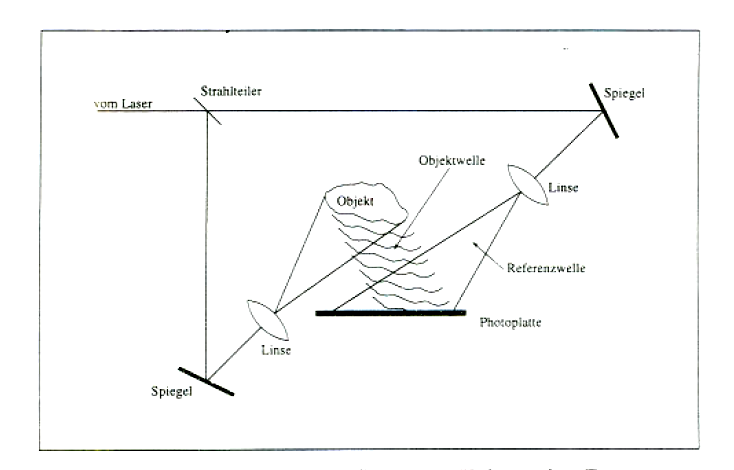
\includegraphics[width=0.5\textwidth]{../figures/holo1}
	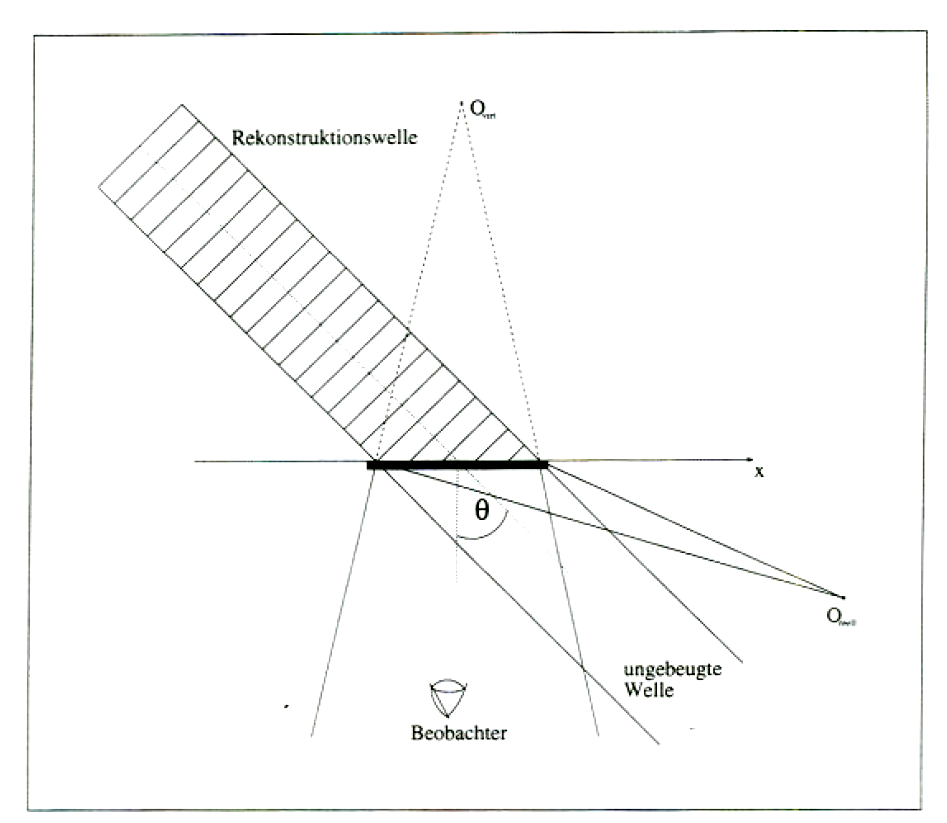
\includegraphics[width=0.4\textwidth]{../figures/holo2}
	\captionof{figure}[Principles of Holography]{left: Set-up to record a Hologram Right: Set up to study a Hologram }
\end{minipage}\vskip 0.5cm



\paragraph{Hologram of a Point}

The holography of a real object can be treated as a ``point cloud'' which means a good understanding of the hologram of a point is fundamental to understand the composition of the hologram of the actual object. 

Let the object wave be a spherical wave that has a certain point $A$ as origin:


\begin{align}
A_1(r)=E_1(r) \ e^{ikr}
\end{align}


The reference wave is a plane wave of the following form:

\begin{align}
A_2(r)=E_2\ e^{ikx \sin\theta} 
\end{align}


The interference of a plane and a spherical wave yields (as previously discussed in \ref{Interference}):

\begin{align}
I=I_1+I_2+2\sqrt{I_1I_2}\cos(k(r-x\sin\theta))
\end{align}



For $\theta=0\degree$ we obtain an interference pattern made up of multiple circular rings. For  $\theta\neq0\degree$ the interference pattern is distorted, the rings won't be of circular shape.



When the hologram is lit with the reconstruction wave
\begin{align}
A_R(r)=A_R\ e^{ikx \sin\theta},
\end{align}


the time independent component carrying the image information of the electric field is given by:


\begin{align}
A(r)=T_AA_R(r)
\end{align}


where $T_A$ is the amplitude transmission of the photo plate that is calculated by:


\begin{align}
T_A=T_0-Ct_BI
\end{align}


with
$T_0$ and $C$ being constants. $t_B$ denotes the exposure time and $I$ denotes the intensity.
This finally yields the following formula:

\begin{align}
A(r)=\underbrace{[T_0-Ct_B(I_1+I_2)]A_R\ e^{ikx \sin\theta}}_{\mbox{no information}} - \underbrace{\sqrt{I_1I_2}A_RCt_B\ e^{ikr}}_{\mbox{vitual image}} - \underbrace{\sqrt{I_1I_2}A_RCt_B\ e^{-ikr}e^{2ikx \sin\theta}}_{\mbox{real image}}
\end{align}



\begin{itemize}
	\item The first term describes a plane not carrying any relevant information
	\item The second term describes the virtual image as it corresponds to the object wave apart from a varying intensity. When studying the virtual image through the hologram it will be located at the position of the object point $A$.
	\item The third term describes the real image.
\end{itemize}

\subsection{Types of Holograms}

In this section we will discuss the different types of holograms feasible.

\subsubsection{Area and Volume Holograms}

As the photo plate on which the grid for the hologram is formed is not infinitely thin, waves advance into the holography medium interfering in the plate. Thus the grid is not limited to a two dimensional surface, it can be considered three dimensional. As a result, only a certain wavelength hitting the plate in the right angle will reflect to an intensity maximum, similar to Bragg reflexion on a lattice. Seeing that holography only uses laser light of one specific wavelength, the hologram needs to be in the same angle to the reconstruction wave as it was to the reference wave when recording the hologram to reconstruct the object.
We speak of an Area Hologram if the thickness of the plate is of the same order of magnitude as the  wavelength of the light source and of a Volume Hologram if it is much bigger.


\subsubsection{Amplitude- and Phase Holograms}

There are two different types of diffraction gratings: Amplitude gratings and Phase gratings. Amplitude gratings have certain spots allowing light to pass through and others that block it off. As a consequence the amplitude, and thereby the intensity of the light wave, is reduced. Phase gratings on the other hand have different optical densities or different refractive indexes causing phase modulation little effecting the intensity.
The same distinction is feasible for holograms by varying the development technique. In order to achieve an amplitude hologram the silver formed during the development is simply fixed. Bleaching the hologram will turn the silver into a transparent silver halogen effectively transforming the amplitude hologram to a phase hologram. 

\subsubsection{Reflection- and Transmission Holograms \label{ReflTrans}}

During the exposure of the photo plate it is possible to let the object and the reference beam incide from the same side, which we call a transmission hologram, as well as from opposite sides, which we call a reflection hologram. (see figure \ref{RTH1})The alignment of the beams chosen determines from which side one has to study the hologram later to observe the reconstructed image of the object.
As the name suggests a transmission hologram needs to be studied with transmitting light (from the side opposite the inciding reference beam). Likewise a reflection hologram has to be studied in reflected light.

\graX[0.7]{Reflex_Transmissions_Hologram}{Comparison of Reflection and Transmission Hologram}{Comparison of Reflection and Transmission Hologram: a) Recording of a Transmission Hologram b) Recording of a Reflection Hologram c) Studying a Transmission Hologram d) Studying a Reflection Hologram \label{RTH1} \cite{staats}}


\subsection{Holographic Interferometry}

A very precise method to measure small changes in objects and make them visible is the holographic interferometry. The underlying basic principle is to compare the hologram of an object with the hologram of the object in a different state or with the object in a different state itself. Three different types of holographic interferometry, namely Double exposure method, time average method and real time method are described below.

\subsubsection{Double exposure holography}

The double exposure method consists of recording the holograms of the object in two different states on the same photo plate. The exposure time should be the same for both states, so the photo plate is ``double exposed'' giving this method its name. Blocking the object beam and studying the hologram created will then reveal and interference pattern of the two states of the object. This method is used to determine the elastic modulus of various materials in this experiment (see \ref{DEH}).

\subsubsection{Real Time holography}

A hologram of an object at rest is recorded, which is then interfered in ``real time'' with the object making it possible to analyze  and reconstruct movements of an object. This method is highly sensitive to disturbances and it is very important for the set-up to not be moved or changed during the process. 

\subsubsection{Time average holography}

This method has the same underlying principle as real time holography with the difference being that here rather fast processes are observed that the human eye or a camera can't resolve. Effectively, only the spatial component is of significance and observed while the temporal component of the movement is neglected. We use this method to determine resonance frequencies of an aluminum plate (see \ref{RTH}).



\subsection{Elastic Modulus of a Beam \label{EMB}}

A horizontal beam, that is clamped on one side can be considered as multiple layers on top of one another. When this beam deformed by a force acting on it,there will be a middle layer which length stays constant while all other layers will either be stretched or compressed (see figure \ref{beam}).

In the following we will consider a beam of length $a$, width $b$ and depth $c$. We now introduce a reference frame in which the x-axis points in the direction of the length of the beam and a force acts on the beam in negative z-direction.\\

As a result of the deformation two cross sections with the distance $dx$ will be in the angle $d\alpha$ to one another. For the length $l$ of a layer in distance $z$ to the middle neutral layer we therefore obtain the following relation:

\begin{align}
l=(r+z)d\alpha
\end{align}


and for the relative change in length this leads to

\begin{align}
\frac{(r+z)d\alpha-r d\alpha}{dx}=z\frac{d\alpha}{dx}=\frac{z}{r} \label{1}
\end{align}


The elastic modulus of the beam is defined as

\begin{align}
\frac{\Delta l}{l}=\frac{1}{E}\frac{dF}{dzdy} \label{2}
\end{align}


Identifying the previous two relations \ref{1} and \ref{2} with one another yields

\begin{align}
dF=\frac{zE}{r}dzdy
\end{align}

This force cause a momentum compensating the force at the end of the beam ($x=a$). For small deformations we obtain the differential equation

\begin{align}
\frac{d^2z}{dx^2}=-\frac{12F}{Ebc^3}(a-x)
\end{align}

Double Integration finally leads to the following relation:

\begin{align}
z=-\frac{12F}{Ebc^3}\left(\frac{ax^2}{2}-\frac{x^3}{6} \right)
\end{align}

\graX[0.7]{balken_biegen}{Elastic Modulus of a Beam}{Deformation of a Beam \cite{staats} \label{beam}}

\subsection{Oscillations of an Aluminium Plate \label{Oscillations}}

Aluminum plate with a speaker behind it causing it to oscillate can be considered as driven harmonic oscillator. In the following we want to outline the calculation of the resonant frequencies, exact calculations are too complex to discuss here and can be found in \cite{staats}.
The starting point to derive an equation describing its behavior is the following differential equation:

\begin{align}
\frac{\partial^2 u}{\partial t^2}+\frac{h^2E}{12\rho(1-\mu^2)}\nabla u=0
\end{align}

where $\Delta$ denotes the Laplace-Operator, $h$ denotes the thickness of the plate and $\rho$ its density respectively while $\mu$ is the poisson number of the plate and $E$ its elastic modulus.

Solving this equation yields:

\begin{align}
f_{m\nu}=\frac{x_{m\nu}^2h}{2\pi R^2}\sqrt{\frac{E}{12\rho(1-\mu^2)}} \label{resfreq}
\end{align}

The $x_{m\nu}$ values are the numerical solution to the following equation:

\begin{align}
J_m(ix)\left[ J_{m-1}(x) - J_{m+1}(x)  \right]  - iJ_m(x)\left[ J_{m-1}(ix) - J_{m+1}(ix)  \right] = 0
\end{align}

with $J$ denoting the Bessel functions of the first kind. Solving these equation (which was done using Mathematica) for $x_{m\nu}$ and then subbing this in in \ref{resfreq} gives the results as seen in Table \ref{tab:eigen} with the following values:

\begin{itemize}
	\item $ R = (5.0\pm0.5)\,\mathrm{cm}$
	\item $h=5\,\mathrm{mm}$
	\item $E=70\,\mathrm{GPa}$
	\item $\rho = 2700\,\frac{\mathrm{kg}}{\mathrm{m^3}}$
	\item $\mu = 0.34$ 
\end{itemize} 

\begin{table}[h]
\centering
	\begin{tabular}{c|c|c}
		Mode 		& $x_{m\nu}$ & Calculated Frequency [Hz] 	 \\ \hline\hline
		$m=0,\nu=0$	&$3.19622$   &$5082$						\\ \hline
		$m=1,\nu=0$	& $4.61090$  & $10577$					\\ \hline
		$m=0,\nu=1$	& $6.30644$  & $19787$					\\ \hline
		$m=2,\nu=0$	& $5.90568$  & $17352$					\\ \hline
		$m=2,\nu=1$	& $9.19688$  & $42081$					\\ \hline
		$m=1,\nu=1$	& $7.79927$  & $30263$				     \\ \hline
		$m=3,\nu=0$	& $7.14353$  & $25388$                \\ \hline
     	$m=3,\nu=1$	& $10.53670$ & $55235$
	\end{tabular} \vskip 0.2cm
	\caption{Calculated eigenfrequencies of the aluminium plate}
	\label{tab:eigen}
\end{table}





\subsection{Working principles of the experimental apparatus}

\subsubsection{Helium-Neon-Laser \label{HeNe1}}

A cavity with partially transparent mirrors is filled with helium and neon gas with a ratio about 10:1. Applying high voltages can achieve ``pumping'' of Helium atoms (pumping medium) to higher energy levels which can than transfer their energy to Neon Atoms (laser medium) by colliding with them. They then get excited to a higher energy level that has a relatively long life time due to forbidden dipole transitions causing population inversion.
The Helium atoms return to the ground state emitting two photons by stimulated emission. Spontaneous emission is suppressed due to the long life time of the excited state. It is important to generate the first stimulated emissions when turning on the laser though.
The energy level system of a Helium-Neon laser is displayed in figure \ref{HeNe}. A helium-Neon laser typically has a wavelength of $632.8\,\mathrm{nm}$.

\graX[0.5]{HeNe}{Energy level system Helium Neon Laser}{Functioning principle of the Helium Neon laser: Energy level system and population inversion for pumping and lasing medium \label{HeNe} \footnotemark}\footnotetext{https://lp.uni-goettingen.de/get/text/1804}


\subsubsection{Spatial Filters \label{SF}}

Spatial Filters are used to filter laser light. Undesired noise and interference or diffraction effects caused by dust or dirt as well as higher frequencies can be eliminated by the beam passing through a lens with a very small focal length followed py a pinhole with a diameter of few micrometers. If the desired output beam is supposed to be a parallel beam which is often the case, a second lens is placed behind the pinhole in the distance of the sum of both focal lengths from the first lens. Without the second lens we obtain a spherical wave. The set-up of a spatial filter is illustrated in figure \ref{SF1}. Spatial Filters can be quite difficult to align in a set-up due to the small focal length of the lens and small diameter of the pinhole (see \ref{DEH}).

\graX[0.5]{SpatialFilter}{Spatial Filter}{Set-Up of a Spatial Filter \label{SF1}}

%\subsubsection{Holographic Medium}

\subsubsection{Pockels Cell}

Pockel cells are voltage-controlled wave plates. Their operational principle is the Pockels effect as the name suggests. The Pockels effect describes the change of the refracting properties of an opitical medium induced by an electric field, namely altering or causing birefringence which is the property of a medium to have a refractive index depending on the polarization of light and/or the propagation direction of light. It is often quantified by the maximum difference of refractive indexes inherit to a material. The applications of a Pockels cell are numerous. For example it can create a fast shutter, able to alternate between ``open'' and ``close'' in nanoseconds, by varying the optical rotation between $0\degree$ and $90\degree$. Furthermore it can also be used to pulse a laser by preventing the optical feedback with a polarizing prism preventing optical amplification by directing light of a specific polarization out of the resonator. This results in the gain medium to being pumped in a highly excited state. When it saturates in energy the Pockels cell is switched reinstating optical feedback leading to all energy built up being very quickly released in form of a light pulse of very high intensity. This is known as active Q-switching.
The Pockels cell is crucial for the observation of the resonant frequencies of the aluminium plate in the third part of the experiment where the laser needs to be pulsed with a similar pulse seperation as the time period of the oscillations.




